\documentclass{standalone}
\usepackage{tikz}
\usepackage{amsmath}
\usetikzlibrary{decorations.pathreplacing}
\usetikzlibrary{calc}
\usetikzlibrary{angles, quotes}

\begin{document}
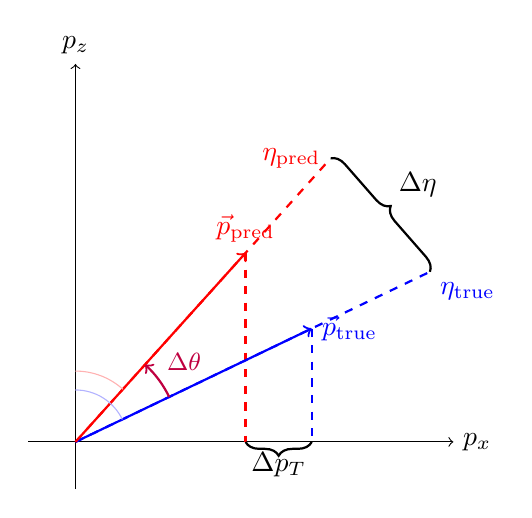
\begin{tikzpicture}[scale=1.2]

    % Axes
    \draw[->] (-0.5,0) -- (4,0) node[right] {$p_x$};
    \draw[->] (0,-0.5) -- (0,4) node[above] {$p_z$};

    \coordinate (origin) at (0,0);
    \coordinate (true) at (2.5,1.2);
    \coordinate (pred) at (1.8,2.0);
    \coordinate (true_pt) at (2.5,0);
    \coordinate (pred_pt) at (1.8,0);

    % True vector
    \draw[thick,blue,->] (origin) -- (true) node[right] {$\vec{p}_{\text{true}}$};
    % Predicted vector
    \draw[thick,red,->] (origin) -- (pred) node[above] {$\vec{p}_{\text{pred}}$};

    % show pt projections
    \draw[thick,blue,dashed] (true) -- (true_pt);
    \draw[thick,red,dashed] (pred) -- (pred_pt);
    \draw[decorate,decoration={brace,amplitude=5pt}, thick] (true_pt) -- (pred_pt) node[midway,below] {$\Delta p_T$};

    % Draw eta lines (extended beyond the vectors)
    \draw[thick, dashed, blue] (origin) -- ($(origin)!1.5!(true)$) node[below right] {$\eta_{\text{true}}$};
    \draw[thick, dashed, red]  (origin) -- ($(origin)!1.5!(pred)$) node[left]        {$\eta_{\text{pred}}$};

    % Brace between the two eta-line endpoints to show Delta eta
    \draw [decorate,decoration={brace,amplitude=5pt,mirror}, thick]
        ($(origin)!1.5!(true)$) -- ($(origin)!1.5!(pred)$)
        node[midway, above right=3pt] {$\Delta \eta$};

    % Arc between the two eta directions showing the angular difference Delta theta
    % true angle from +px axis:  atan2(1.2, 2.5) = 25.64 deg
    % pred angle from +px axis:  atan2(2.0, 1.8) = 48.01 deg
    \draw[thick, purple, ->]
        ($(origin)!1.1cm!(true)$)
        arc[start angle=25.64, end angle=48.01, radius=1.1cm];
    \node[purple] at (1.15, 0.85) {\small $\Delta\theta$};

    % Reference angle arc from beam axis (p_z axis) to the true eta line
    % p_z is at 90 deg; true vector is at 25.64 deg from px, so from pz it is 90-25.64=64.36 deg
    \draw[blue!30!white, thin]
        (0, 0.55cm)
        arc[start angle=90, end angle=25.64, radius=0.55cm];

    \draw[red!30!white, thin]
        (0, 0.75cm)
        arc[start angle=90, end angle=48.01, radius=0.75cm];


\end{tikzpicture}
\end{document}